\section{Deep Information Propagation in DGN}\label{sec:optimisation}
In this section, we study deep information propagation (DIP) in DGNs when the gates are frozen, i.e., $\G_t=\G_0,\forall t\geq 0$, and our results are applicable to the following:

(i) \emph{Deep Linear Networks (DLN):} where, all the gating values are $1$. Here, since all the paths are \emph{always on}, we do not have any control over how the paths are formed.

(ii) \emph{Fixed random gating (DGN-FRG):} Note that $\G_0$ contains $n\times (d-1)\times w$ gating values, corresponding to the $n$ input examples, $(d-1)$ layer outputs and $w$ nodes in each layer. In DGN-FRG, $\G_0\in \{0,1\}^{n\times (d-1)\times w}$, where each gating value is chosen to be $0$ or $1$ with probabilities $1-p$ and $p$ respectively. Here, we have full control over the gating/activation level of the paths. These networks are restricted solely towards understanding questions related to optimisation. Generalisation is irrelevant for DGN-FRG networks because there is no natural means to extend the random gate generation for unseen inputs.

(iii) \emph{Gated linear unit (GaLU):} networks, wherein the gating values are generated by \emph{another separate} network which is DNN with ReLU gates. Unlike DGN-FRG, GaLU networks can generalise.

We first express the Gram matrix $K_t$ in the language of the paths. We then state our assumption in Assumption~\ref{assmp:mainone},~\ref{assmp:maintwo} followed by our main result on deep information propagation in DGNs (\Cref{th:dgnexp}). We then demonstrate how our main result applies to DGN-FRG and GaLU networks.\footnote{DLN discussion has been moved to the Supplementary Material in the end.}

When the gates are frozen, the weight update affects only the path strengths $w_t(p),p\in[P]$. This is captured as follows:

\textbf{Sensitivity of the path strength}: Let $p\in[P]$ be a path, and $w_t(p)$ be its strength at time $t$. Further, let $\theta(m),m\in[d_{net}]$ be a weight and without loss of generality, let $\theta(m)$ belong to layer $l'(m)\in[d]$. At time $t$, the derivative of path $p$ with respect to $\theta(m)$ denoted by $\varphi_{t,p}(m)$ is given by:
\begin{align}
\begin{split}
\varphi_{t,p}(m)&=\underset{l\neq l'(m)}{\underset{l=1}{\overset{d}{\Pi}}} \Theta_t(l,p(l-1),p(l)), \forall p\rsa\theta(m),\\
\varphi_{t,p}(m)&=0, \forall p\bcancel{\rsa}\theta(m)
\end{split}
\end{align}
The sensitivity of a path $p$ with respect to $\Theta_t\in\R^{d_{net}}$ is then given by the vector $\varphi_{t,p}=(\varphi_{t,p}(m),m\in[d_{net}])\in \R^{d_{net}}$.

\begin{lemma}[Signal vs Wire Decomposition]\label{lm:sigwire}
Let $\kappa_t(s,s',i)\stackrel{def}=\underset{p_1,p_2\rsa i}{\sum_{p_1,p_2\in P:}} A_{\G_t}(x_s,p_1) A_{\G_t}(x_{s'},p_2) \ip{\varphi_{t,p_1}, \varphi_{t,p_2}}$. The Gram matrix $K_t$ is then given by 
\begin{align}\label{eq:ktalg}
{K_t(s,s')}=\sum_{i=1}^{d_{in}} x(i,s)x(i,s') \kappa_t(s,s',i)
\end{align}
\end{lemma}
In Lemma~\ref{lm:sigwire}, $\kappa_t(s,s',i)$ is the amount of overall interaction within the DGN in the $i^{th}$ dimension of inputs $x_s,x_{s'}\in \R^{d_{in}}$. Note that, thanks to the path-view, the `signal', i.e., $x_s(i)x_{s'}(i)$ gets separated from the `wire', i.e., the connections in the DGN, which is captured in the `$\kappa_t$' term. Further, the algebraic expression for $K_t$ in \eqref{eq:ktalg} applies to all DGNs (including the standard DNN with ReLU activations).

\textbf{Simplifying $\kappa$}, which contains the joint path activity given by $A(x_s,p_1)A(x_{s'},p_2)$, and the inter-path interaction given by $\ip{\varphi_{t,p_1}, \varphi_{t,p_2}}$, is the next step. Towards this end, we state and discuss Assumptions~\ref{assmp:mainone},~\ref{assmp:maintwo}.
\begin{assumption}\label{assmp:mainone}
$\Theta_0\stackrel{iid}\sim Ber\left(\frac{1}{2}\right)$ over the set $\{-\sigma,+\sigma\}$. 
\end{assumption}
\textbf{Decoupling of paths from one another}, which stands for the fact that the inner product $\ip{\varphi_{t,p_1}, \varphi_{t,p_2}}$ of two different paths $p_1,p_2$ is $0$ on expectation. This is captured in Lemma~\ref{lm:pathdot} below.
\begin{lemma}\label{lm:pathdot}
Under Assumption~\ref{assmp:mainone}, for paths $p,p_1,p_2\in \P, p_1\neq p_2$, at initialisation we have (i) $\E{\ip{\varphi_{0,p_1}, \varphi_{0,p_2}}}= 0$, (ii) ${\ip{\varphi_{0,p}, \varphi_{0,p}}}= d\sigma^{2(d-1)}$
\end{lemma}

\begin{assumption}\label{assmp:maintwo}
$\G_0$ is statistically independent of $\Theta_0$.
\end{assumption}
\textbf{Decoupling of gates and paths:} In a standard DNN with ReLU activations, the gating and path strengths are statistically dependent, because, conditioned on the fact that a given ReLU activation is \emph{on}, the incoming weights of that activation cannot be simultaneously all \emph{negative}. Assumption~\ref{assmp:maintwo} makes path strength statistically independent of path activity.

\begin{theorem}[DIP in DGN]\label{th:dgnexp}
Under Assumption~\ref{assmp:mainone}, ~\ref{assmp:maintwo}, and $\frac{4d}{w^2}<1$ it follows that
 \begin{align*}
&\E{K_0}=d\sigma^{2(d-1)}(x^\top x \odot \lambda_0)\\
&Var\left[K_0\right]\leq O\left(d^2_{in}\sigma^{4(d-1)}\max\{d^2w^{2(d-2)+1}, d^3w^{2(d-2)}\}\right)
\end{align*}
\end{theorem}

\textbf{Choice of $\sigma$:} Note that, in the case of gates taking values in $\{0,1\}$, $\lambda_0(s,s'), s,s'\in [n]$ is a measure of overlap of sub-networks that start at any given input node, end at the output node, and are active for both input examples $s,s'$.
Loosely speaking, say, in each layer $\mu\in(0,1)$ fraction of the gates are \emph{on}, then $\lambda_0(s,s)$ is about $(\mu w)^{d-1}$. Thus, to ensure that the signal does not blow up in a DGN, we need to ensure $(\sigma^2 \mu w)^{d-1}=1$, which means $\sigma=O\left(\sqrt{\frac1{\mu w}}\right)$. %In our experiments, we set $\sigma=\sqrt{\frac{2}{w}}$.

In the expression for $\E{K_0}$, note that the input Gram matrix $x^\top x \in \R^{n\times n}$ is separate from $\lambda_0\in \R^{n\times n}$,	 which is a Gram matrix of the active sub-networks. Thanks to the path-view, we do not lose track of the input information, which, is otherwise bound to happen if we were to choose a layer by layer view of DIP in DGNs.

\begin{figure*}
\resizebox{\textwidth}{!}{
\begin{tabular}{ccc}
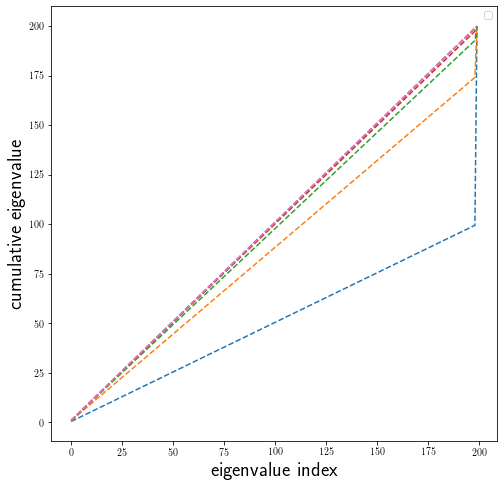
\includegraphics[scale=0.4]{figs/dgn-fra-ecdf-ideal.png}
&
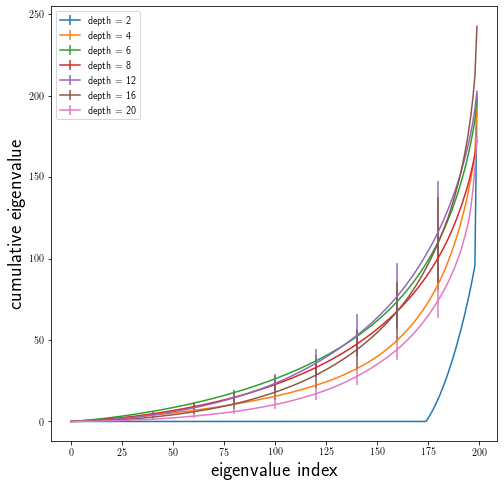
\includegraphics[scale=0.4]{figs/dgn-fra-ecdfbyd-w25.png}
&
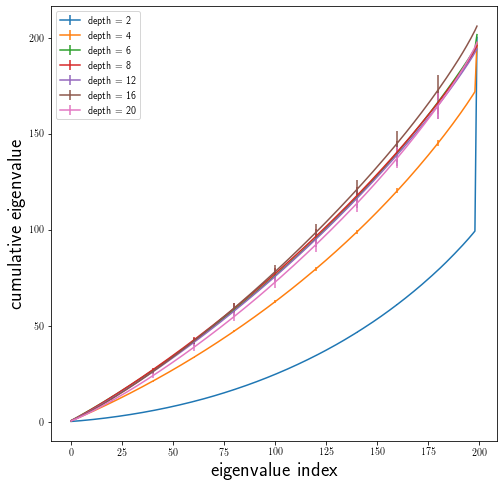
\includegraphics[scale=0.4]{figs/dgn-fra-ecdfbyd-w500.png}
\end{tabular}
}
\caption{Shows the plots for DGN-FRG with $\mu=\frac{1}{2}$ and $\sigma=\sqrt{\frac{2}{w}}$. The first plot in the left shows the ideal cumulative eigenvalue (e.c.d.f) for various depths $d=2,4,6,8,12,16,20$. Note that the ideal plot converges to identity matrix as $d$ increases. The second and third plot (from the left),  
plots respectively show the cumulative eigenvalues (e.c.d.f) for $w=500$ and $w=25$ respectively. Note that the e.c.d.f of higher width $w=500$ is better conditioned than the e.c.d.f of $w=25$.}
\label{fig:dgn-frg-gram-ecdf}
\end{figure*}



\textbf{Fixed Random Gating (DGN-FRG)} involves sampling the gates $\G_0$ from $Ber\left(\mu\right)$, and hence there is a random sub-network which is active for each input. Under FRG, we can obtain closed form expression for the `$\lambda(\cdot,\cdot,\cdot)$' term as below:

\begin{lemma}\label{lm:dgn-fra}  
 Under Assumption~\ref{assmp:mainone},~\ref{assmp:maintwo} and gates sampled iid $Ber(\mu)$, we have, $\forall s,s'\in[n]$

(i) $\mathbb{E}_p\left[\lambda_0(s,s)\right]=\bar{\lambda}_{self}=(\mu w)^{d-1}$

ii) $\mathbb{E}_p\left[\lambda_0(s,s')\right]=\bar{\lambda}_{cross}= (\mu^2w)^{d-1}$
\end{lemma}

\textbf{DIP in DGN-FRG:} For $\sigma=\sqrt{\frac{1}{\mu w}}$, we have:

\begin{align*}
\frac{\E{K_0}}{d}=\left[\begin{matrix}
\cdot&\cdot &\cdot &\cdot &\cdot \\ 
\cdot&\ip{x_s,x_s}\quad\quad &\cdot &\quad\quad\ip{x_s,x_{s'}}\mu^{d-1} &\cdot\\ 
\cdot&\ip{x_{s'},x_s}\mu^{d-1} &\cdot &\ip{x_{s'},x_{s'}} &\cdot \\
\cdot&\cdot &\cdot &\cdot &\cdot  
\end{matrix}\right]
\end{align*}


\textbf{Experiment $1$:} Consider the dataset $(x_s,y_s)_{s=1}^n\in \R\times \R$, where $x_s=1,\forall s\in [n]$, and $y_s\sim unif([-1,1])$, $n=200$. The input Gram matrix $x^\top x$ is a $n\times n$ matrix with all entries equal to $1$ and its rank is equal to 1. Since all the inputs are identical, this is the worst possible case for optimisation.


\textbf{Why increasing depth till a point helps ?} 
In the case of \textbf{Experiment $1$}, we have:

\begin{align}\label{eq:mat}
\frac{\E{K_0}}{d}=\left[\begin{matrix}
1 &\mu^{d-1} &\ldots &\mu^{d-1} &\ldots\\ 
\ldots &1 &\ldots &\mu^{d-1} &\ldots\\ 
\ldots &\mu^{d-1} &\ldots &1 &\ldots \\
\ldots &\mu^{d-1} &\ldots &\mu^{d-1} &1\\ 
\end{matrix}\right]
\end{align}

i.e., all the diagonal entries are $1$ and non-diagonal entries are $\mu^{d-1}$. Now, let $\rho_i\geq 0,i \in [n]$ be the eigenvalues of $\frac{\E{K_0}}{d}$, and let $\rho_{\max}$ and $\rho_{\min}$ be the largest and smallest eigenvalues. From the structure of \eqref{eq:mat}, one can easily show that $\rho_{\max}=1+(n-1)\mu^{d-1}$ and corresponds to the eigenvector with all entries as $1$, and $\rho_{\min}=(1-\mu^{d-1})$ repeats $(n-1)$ times, which corresponds to eigenvectors given by $[0, 0, \ldots, \underbrace{1, -1}_{\text{$i$ and $i+1$}}, 0,0,\ldots, 0]^\top \in \R^n$ for $i=1,\ldots,n-1$.



\textbf{Why increasing depth beyond a point hurts?} 
In \Cref{th:dgnexp}, note that for a fixed width $w$, as the depth increases, the variance of $K_0(s,s')$ increases, and hence the entries of $K_0$ deviates from its expected value $\E{K_0}$. Thus the structure of the Gram matrix degrades from \eqref{eq:mat}, leading to smaller eigenvalues.

\textbf{Numerical Evidence (Gram Matrix):} We fix arbitrary diagonal and non-diagonal entries, and look at their value averaged over $20$ run (see \Cref{fig:dgn-frg-gram-diag}). The actual values shown in bold indeed follow the ideal values shown in the dotted lines and the values are as per \eqref{eq:mat}). 


\begin{figure}[h]
\resizebox{\columnwidth}{!}{
\begin{tabular}{cc}
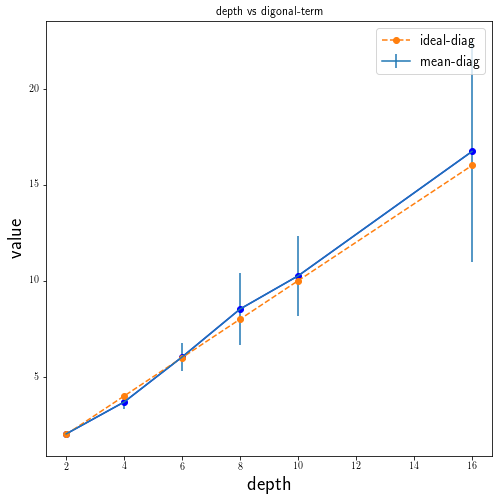
\includegraphics[scale=0.4]{figs/dgn-frg-diag.png}
&
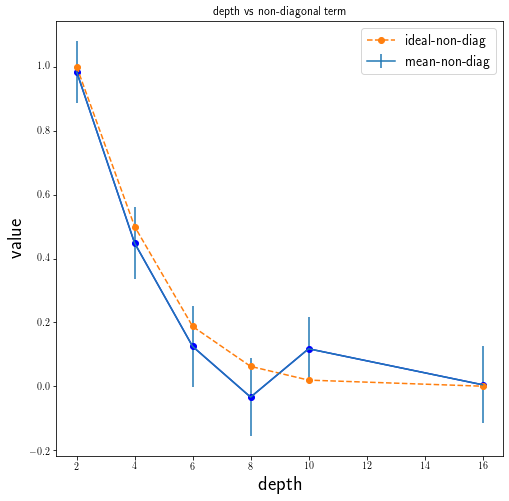
\includegraphics[scale=0.4]{figs/dgn-frg-non-diag.png}
\end{tabular}
}
\caption{For $w=500$, and $\mu=0.5$, (an arbitrary) diagonal (left plot) and non-diagonal (right plot) of the Gram matrix $K_0$ for dataset in Experiment~$1$ is shown. The plots are averaged over $20$ runs.}
\label{fig:dgn-frg-gram-diag}
\end{figure}


\textbf{Numerical Evidence (Spectrum):} 
Next, we look at the cumulative eigenvalue (e.c.d.f) obtained by first sorting the eigenvalues in ascending order then looking at their cumulative sum. The ideal behaviour (middle plot of \Cref{fig:dgn-frg-gram-ecdf}) as predicted from theory is that for indices $k\in[n-1]$, the e.c.d.f should increase at a linear rate, i.e., the cumulative sum of the first $k$ indices is equal to $k(1-\mu^{d-1})$, and the difference between the last two indices is $1+(n-1)\mu^{d-1}$. In \Cref{fig:dgn-frg-gram-ecdf}, we plot the e.c.d.f for various depths $d=2,4,6,8,12,16,20$ and two different width namely $w=25,500$. It can be seen that as $w$ increases, the difference between the ideal and actual e.c.d.f curves is less ($w=500$ when compared to $w=25$).

\textbf{Numerical Evidence (Role of Depth):} 
In order to compare how the rate of convergence varies with the depth in DGN-FRG network, we set the step-size $\alpha=\frac{0.1}{\rho_{\max}}$, $w=100$, and fit the data described in \textbf{Experiment $1$}. We use the vanilla SGD-optimiser. Note that if follows from \eqref{eq:basictraj} that the convergence rate is determined by a linear recursion, and choosing $\alpha=\frac{0.1}{\rho_{\max}}$ can be seen to be equivalent to having a constant step-size of $\alpha=0.1$ but dividing the Gram matrix by its maximum eigenvalue instead. Thus, after this rescaling, the maximum eigenvalue is $1$ uniformly across all the instances, and the convergence should be limited by the smaller eigenvalues. We also look at the convergence rate of the ratio $\frac{\norm{e_t}^2_2}{\norm{e_0}^2_2}$, and we observe that the convergence rate gets better with depth as predicted by theory (\Cref{fig:dgn-frg}).

\begin{figure*}
\resizebox{\textwidth}{!}{
\begin{tabular}{cccc}

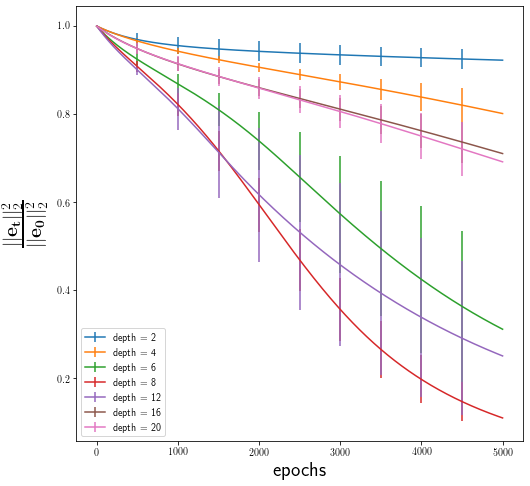
\includegraphics[scale=0.4]{figs/dgn-fra-conv-w25.png}
&
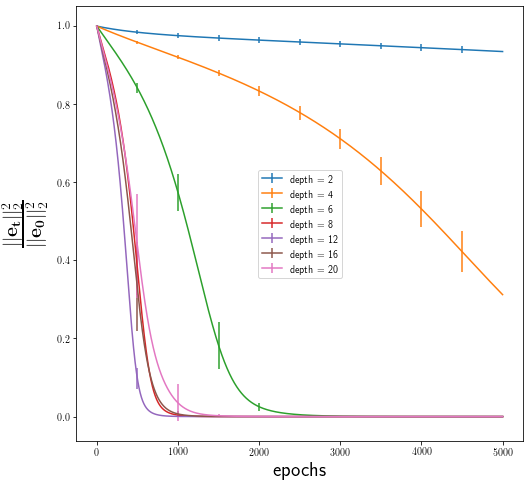
\includegraphics[scale=0.4]{figs/dgn-fra-conv-w500.png}
&
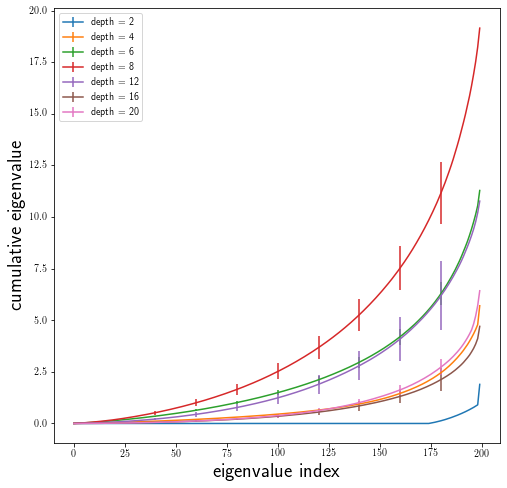
\includegraphics[scale=0.4]{figs/dgn-fra-ecdfbymax-w25.png}
&
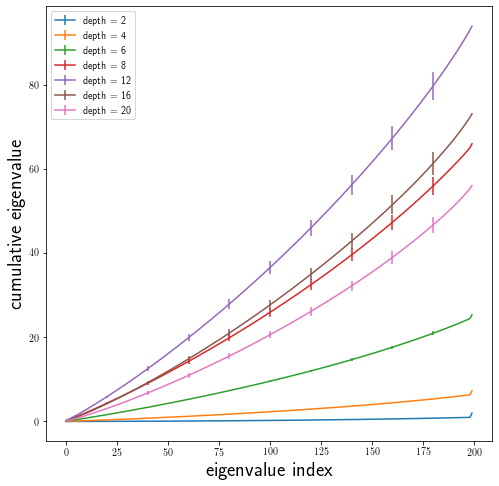
\includegraphics[scale=0.4]{figs/dgn-fra-ecdfbymax-w500.png}
\end{tabular}
}
\caption{Shows the plots for DGN-FRG. The left two plots show the convergence rates for $w=25$ and $w=500$. The right two values are showing the e.c.d.f obtained by first dividing the Gram matrix by their maximum eigenvalue. The plots are averaged over $5$ runs.}
\label{fig:dgn-frg}
\end{figure*}
\begin{figure*}
\resizebox{\textwidth}{!}{
\begin{tabular}{cccc}
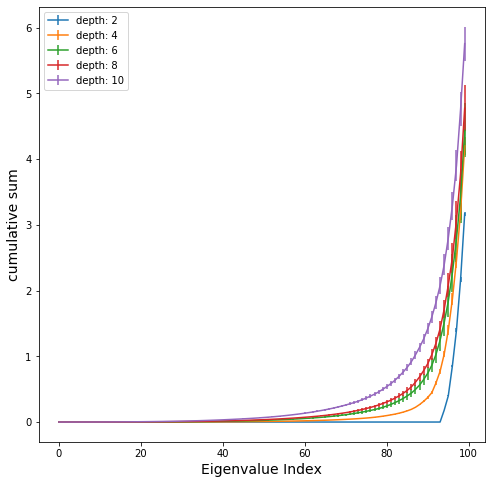
\includegraphics[scale=0.4]{figs/galu-ecdf-d.png}
&
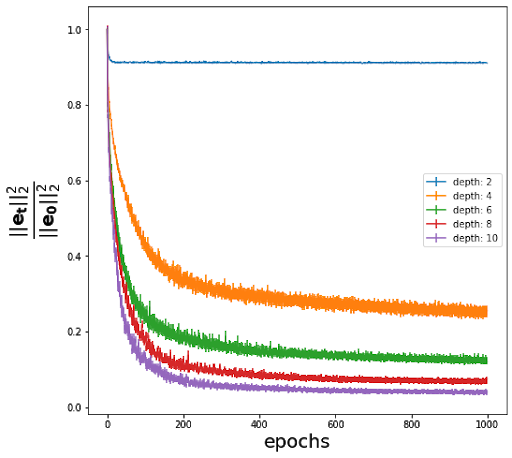
\includegraphics[scale=0.4]{figs/galu-conv-d.png}
&
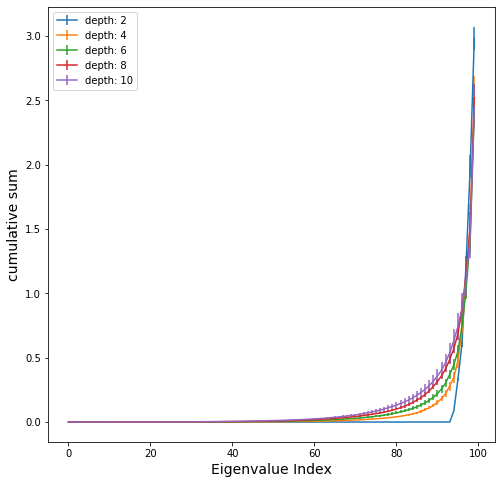
\includegraphics[scale=0.4]{figs/relu-ecdf.png}
&
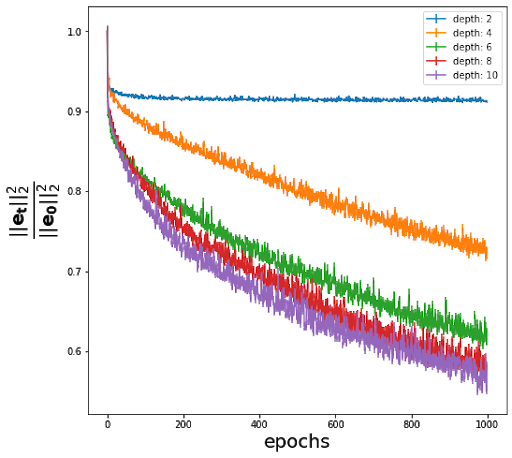
\includegraphics[scale=0.4]{figs/relu-conv.png}
\end{tabular}
}
\caption{The left two plots shows the e.c.d.f and convergence rates for various depth in GaLU networks $w=100$. The third and fourth plot from the left show the e.c.d.f and convergence rates for various depth in ReLU networks $w=100$. The plots are averaged over $5$ runs. }
\label{fig:galu-d}
\end{figure*}

\textbf{GaLU Networks:} Here, the gating values are obtained from a DNN with ReLU activation, parameterised by $\Tg\in \R^{d_{net}}$ (these weights are frozen). Now, let us define $\bar{\lambda}_{self}(s)\stackrel{def}=\mathbb{E}_{\Tg_0}\left[\lambda_0(s,s)\right]$, and $\bar{\lambda}_{cross}(s,s')\stackrel{def}= \mathbb{E}_{\Tg_0}\left[\lambda_0(s,s')\right]$. Note that, due to the inherent symmetry in weights (Assumption~\ref{assmp:mainone}) , we can expect roughly half the number of activations to be \emph{on}, and it follows that $\bar{\lambda}_{self}(s)\approx (\mu w)^{d-1}$ with $\mu\approx\frac12$. Also, let $\tau(s,s',l)\stackrel{def}=\sum_{i=1}^w G_{x_s,t}(l,i)G_{x_s',t}(l,i)$,  let $\eta\stackrel{def}=\max_s\left(\max_{s',l} \frac{\tau(s,s',l)}{\tau(s,s,l)}\right)$ be the maximum overlap between gates of a layer (maximum taken over over input pairs $s,s'\in[n]$ and layers $l\in [d]$), then it follows that $\max_{s,s'\in [n]} \frac{\bar{\lambda}_{cross}(s,s')}{\bar{\lambda}_{self}(s)}\leq \eta^{d-1}$. Thus,  we can see that while the non-diagonal entries of the $\E{K_0}$ decay at a different rates, the rate of decay is nonetheless upper bounded by $\eta^{d-1}$. Note that in DGN-FRG decay of non-diagonal terms is at a uniform rate given by $\mu^{d-1}$.



\textbf{Experiment $2$:} To characterise the optimisation performance of GaLU and ReLU networks, we consider the dataset $(x_s,y_s)_{s=1}^{n}\in \R^2\times \R$, where, $x_s\stackrel{iid}\sim unif(\left[-1,1\right]^2)$ and $y_s\stackrel{iid}\sim unif([-1,1])$, $n=100$. The results are shown in \Cref{fig:galu-d}. The rationale behind choosing this data set is that, we want the inputs to be highly correlated by choice.
 
 \textbf{GaLU Networks (Depth helps in training): }The trend is similar to DGN-FRG case, in that, both e.c.d.f as well as convergence get better with increasing depth. Here too we set the step-size $\alpha=\frac{0.1}{\rho_{\max}}$ (and use vanilla SGD). We also observe that in \textbf{Experiment $2$} \emph{GaLU networks optimise better than standard ReLU networks}, and it is also true that the e.c.d.f for the case of GaLU is better than that of ReLU. This can be attributed to the fact that, in ReLU network the dot product of two different active paths is not zero and hence the Gram matrix entries fall back to the algebraic expression for $K_t$ in \eqref{eq:ktalg}.


